%% ****** Start of file aiptemplate.tex ****** %
%%
%%   This file is part of the files in the distribution of AIP substyles for REVTeX4.
%%   Version 4.1 of 9 October 2009.
%%
%
% This is a template for producing documents for use with 
% the REVTEX 4.1 document class and the AIP substyles.
% 
% Copy this file to another name and then work on that file.
% That way, you always have this original template file to use.

%\documentclass[aip,graphicx]{revtex4-1}
%\documentclass[aip,reprint]{revtex4-1}

%\usepackage{graphicx}

%\draft % marks overfull lines with a black rule on the right
\documentclass[pre,aps,floatfix,authordate1-4,twocolumn]{revtex4-1}
%\documentclass[pre,aps,floatfix,authordate1-4]{revtex4-1}

%\documentclass[aps,prl,preprint,superscriptaddress]{revtex4}



%\documentclass[aps,prl,preprint,groupedaddress]{revtex4}

\usepackage{rotating} 
\usepackage{times}
\usepackage{graphicx}
\usepackage{setspace}
\usepackage{amsmath}
\usepackage{epstopdf}
\usepackage[obeyFinal]{easy-todo}
\usepackage{lipsum}
\begin{document}

% Use the \preprint command to place your local institutional report number 
% on the title page in preprint mode.
% Multiple \preprint commands are allowed.
%\preprint{}

\title{Rotational dynamics of proteins from spin relaxation times and molecular dynamics simulations} %Title of paper

% repeat the \author .. \affiliation  etc. as needed
% \email, \thanks, \homepage, \altaffiliation all apply to the current author.
% Explanatory text should go in the []'s, 
% actual e-mail address or url should go in the {}'s for \email and \homepage.
% Please use the appropriate macro for the type of information

% \affiliation command applies to all authors since the last \affiliation command. 
% The \affiliation command should follow the other information.

\author{O. H. Samuli Ollila}
\email[]{samuli.ollila@helsinki.fi}
%\homepage[]{Your web page}
%\thanks{}
\affiliation{Insititute of Biotechnology, University of Helsinki}
\affiliation{Institute of Organic Chemistry and Biochemistry,
Czech Academy of Sciences, 
Prague 6, Czech Republic}

\author{Hideo Iwa\"i}
%\homepage[]{Your web page}
%\thanks{}
\affiliation{Insititute of Biotechnology, University of Helsinki}

% Collaboration name, if desired (requires use of superscriptaddress option in \documentclass). 
% \noaffiliation is required (may also be used with the \author command).
%\collaboration{}
%\noaffiliation

\date{\today}

\begin{abstract}
  % insert abstract here
  Conformational fluctuations and rotational tumbling of proteins can be experimentally accessed
  with nuclear spin relaxation experiments. Interpretation of molecular dynamics from the
  experimental data is, however, often complicated, especially for molecules with anisotropic
  shape. Here we apply classical molecular dynamics simulations to interpret conformational fluctuations
  and rotational tumbling of proteins with arbitrarily anisotropic shape. The direct calculation
  of spin relaxation times from simulation data did not reproduce the experimental data.
  This was successfully corrected by scaling the overall rotational diffusion constants around
  protein intertia axes with a constant factor. The achieved good agreement with experiments
  allowed the interpretation of internal and overall dynamics of proteins with significantly
  anisotropic shape. The overall rotational diffusion was found to be brownian, having only a
  short subdiffusive region below 0.12~ns. The presented methodology can be applied to
  interpret rotational dynamics and conformation fluctuations of proteins with arbitrary anisotropic
  shape. However, for intrinsically disordered proteins a water model with more realistic
  dynamical properties is probably required.
\end{abstract}

%\pacs{}% insert suggested PACS numbers in braces on next line

\maketitle %\maketitle must follow title, authors, abstract and \pacs

% Body of paper goes here. Use proper sectioning commands. 
% References should be done using the \cite, \ref, and \label commands


%\label{}
\section{Introduction}
Conformational fluctuations and entropy of proteins
play a significant role in functionality
and interactions with other biomolecules.
Conformation fluctuations and overall brownian tumbling of proteins
are experimentally accessible through 
spin relaxation times of $^{15}$N and $^{13}$C nucleai measured
with nuclaer magnetic resonance (NMR) 
techniques \cite{jarymowycz06,korzhnev01,mulder01,eisenmesser05,bedem15,lewandowski15,lamley15}. 
Spin relaxation rates have been used to, for example, analyze
conformational entropies \cite{yang96,kasinath13,allner15,jarymowycz06}, binding entropies \cite{akke93,jarymowycz06},
resolve sampled structures \cite{mulder01,eisenmesser05,bedem15,medina14}
and validate molecular dynamics simulations \cite{best04,showalter07a,showalter07b,maragakis08,trbovic08}.
These analyzes are almost exclusively based on the
separation of internal conformational fluctuations 
and overall rotational tumbling \cite{wennerstrom79,Lipari82} and
isotropic overall diffusion is often assumed, while
analysis of anisotropic molecules is significantly more
complicated \cite{woessner62,shimizu62,jarymowycz06,korzhnev01,luginbuhl97,hall04}.
Thus, new approaches are needed to intepret spin relaxation times
measured from anisotropic or intrinsically disordered molecules.


%This approach has been successfully applied for large amount of proteins
%with isotropic shape and overall rotational diffusion \cite{jarymowycz06}.
%The resulting order parameters and overall rotational diffusion coefficients
%
%, however, proteins
%with anisotropic shape or large amount of internal motional timescales
%are 
%proteins parameter space for fitted parameters become
%rotational diffusion and internal flexibility of proteins and other biomolecules.
%On the other hand, segmental level information has been used in validation
%and improvement of molecular dynamics simulation force fields \cite{??}.
%Segmental order has been also related to conformational entropy of proteins \cite{??}.

 
Classical molecular dynamics simulation methods are
promising tools to interpretate spin relaxation experiments
for molecules with significant anisotropy or correlations between
internal and overall rotational motions. Practical applications
are, however, limited by inaccuracies in the force field descriptions
and available time scales in the simulations \cite{prompers02,maragakis08,trbovic08,wong08,anderson12}.
The main issues have been the overestimated overall rotational diffusion of proteins
due to inaccuracies in water models~\cite{wong08} and
insufficient accuracy of correlation functions calculated from
single molecules in MD simulations~\cite{lu06,anderson12}.

In this work we overcome these issues by assuming that the overall
rotational dynamics of protein follows anisotropic rigid body diffusion.
Diffusion coefficients around inertia axes are 
directly calculated from angular displacements.
The diffusion coefficients are then used to determine the
contribution of overall rotational tumbling to the 
N-H bond rotational correlation functions.
This reduces the required simulation length for accurate determination
of rotational correlation functions. Furthermore, the overestimated
overall brownian tumbling rates due to the inaccurate water model
can be corrected during correlation function calculation by scaling
diffusion coefficients in all directions with a constant factor.
The corrected correlation functions can be used to interpret spin relaxation
experiments for proteins with arbitrarily anisotropic shape.

The developed approach is demonstrated by interpreting spin relaxation data 
for C-terminal domains of TonB proteins from {\it H. pyroli} ({\it Hp}TonB)~\cite{ciragan16}
and from {\it Pseudomonas aeruginosa} ({\it Pa}TonB). Both proteins have significantly
anisotropic shape, which would significantly complicate the standard spin relaxation data
analysis~\cite{woessner62,shimizu62,jarymowycz06,korzhnev01,luginbuhl97,hall04}.
%These protein segments are critical for iron transport into Helicbacteri
%Pyroli and Pseudomonas bacteria, respectively.


\section{Methods}

\subsection{Spin relaxation experiments and rotational dynamics of molecules}
Molecular dynamics of protein backbone residues and spin relaxation experiments can
be connected by using the spectral density $J(\omega)$ 
\begin{equation}\label{SPECTdens}
  J(\omega)=2\int_0^\infty C(t) \cos(\omega t) {\rm d}t,
\end{equation}
which is the Fourier transformation of the second order
rotational correlation function for N-H bond vector
\begin{equation}\label{CORRFdef}
  C(t)=\langle \frac{3}{2}\cos^2\theta_{t'+t}-\frac{1}{2} \rangle_{t'},
\end{equation}
where $\theta_{t'+t}$ is the N-H bond angle between times $t'$ and $t'+t$
and angular brackets refer to the ensemble average.
Connection to experimentally measured spin relaxation times $T_1$, $T_2$
and $T_{\rm NOE}$ is given by Redfield equations \cite{abragam,kay89}
\begin{equation}\label{R1}
  \begin{aligned}
  \frac{1}{T_1}= & \frac{d_{\rm{NH}}^2N_{\rm{H}}}{20}\bigg[J(\omega_{\rm{H}}-\omega_{\rm{N}})+3J(\omega_{\rm{N}})+6J(\omega_{\rm{N}}+\omega_{\rm{H}})\bigg] \\
        & +\frac{(\sigma \omega_{\rm{N}})^2}{15}J(\omega_{\rm{N}}),
  \end{aligned}
\end{equation}
\begin{equation}\label{R2}
    \begin{aligned}
  \frac{1}{T_2}= & \frac{1}{2}\frac{d_{\rm{NH}}^2N_{\rm{H}}}{20}\bigg[4J(0)+3J(\omega_{\rm{N}})+J(\omega_{\rm{H}}-\omega_{\rm{N}})+6J(\omega_{\rm{H}})  \\
    & +6J(\omega_{\rm{N}}+\omega_{\rm{H}})\bigg]+\frac{(\sigma \omega_{\rm{N}})^2}{90}[4J(0) +3J(\omega_{\rm{N}})],
    \end{aligned}
\end{equation}
\begin{equation}\label{NOE}
  \frac{1}{T_{\rm NOE}}=1+\frac{d_{\rm{NH}}^2N_{\rm{H}}}{20}\bigg[6J(\omega_{\rm{N}}+\omega_{\rm{H}})+J(\omega_{\rm{H}}-\omega_{\rm{N}}))\bigg]\frac{\gamma_{\rm{H}}T_1}{\gamma_{\rm{N}}},
\end{equation}
where $\omega_{\rm{N}}$ and $\omega_{\rm{H}}$ are the Larmor angular
frequencies of $^{15}$N and $^1$H respectively, and
the number of bound protons $N_{\rm{H}}=1$ for N-H bonds.
The dipolar coupling constant is given by
\begin{equation}
d_{\rm{NH}}=-\frac{\mu_0\hbar\gamma_{\rm{H}}\gamma_{\rm{N}}}{4\pi\langle r_{\rm{CN}}^3\rangle},\nonumber
\end{equation}
where $\mu_0$ is the magnetic constant or vacuum permeability, $\hbar$ is the reduced Planck constant,
$\gamma_{\rm{N}}$ and $\gamma_{\rm{H}}$ are the gyromagnetic constants of $^{15}$N and $^1$H, respectively.
Average cubic length is calculated as $\langle r_{\rm{CN}}^3\rangle = (0.101{\rm nm})^3$ and the 
value of $\Delta \sigma = -160$ ppm is used for the chemical shift anisotropy of N-H bonds in 
proteins \cite{kay89,hiyama88}.
%Same equations can be used, for example, to C-H bond by changing the
%constants related to nitrogen to the ones corresponding carbon. 

Spin relaxation experiments are typically interpreted for proteins by
assuming that the motions related to overall brownian tumbling 
and conformational fluctuations are independent.
The rotational correlation function for chemical bonds can be then written
as  \cite{wennerstrom79,Lipari82,jarymowycz06,korzhnev01,halle09}
\begin{equation}\label{CORRFsep}
  C(t)=C_I(t)C_O(t),
\end{equation}
where $C_I(t)$ and $C_O(t)$ are correlation functions for internal and overall
rotations, respectively. Conformational fluctuations can be described
in this approximation by using the square of order parameter respect to 
molecular axes $S^2$, which is given by the plateau of the internal rotational 
correlation function. Timescales for the fluctuations can be characterized by
using the effective correlation time 
\begin{equation}\label{effCT}
  \tau_{\rm eff}=\int_0^\infty C_I'(t) \mathrm{d}t,
\end{equation}
where $C_I'(t)=\frac{C_I-S^2}{1-S^2}$ is the reduced correlation function \cite{Lipari82}.

The overall rotational correlation function is often described
by approximating a protein as a rigid body.
For arbitrarily anisotropic molecules the correlation functions
can  be then presented as a sum of five exponentials~\cite{woessner62,korzhnev01}
\begin{equation}\label{CORRFanisot}
  C_O(t)=\sum_{j=1}^5 A_j e^{-t/\tau_j},
\end{equation}
where time constants $\tau_j$ are related 
to the diffusion constants around
three principal axes of a molecule
($D_{xx}$, $D_{yy}$ and $D_{zz}$)  
\footnote{
$\tau_1=(4D_{xx}+D_{yy}+D_{zz})^{-1}$,
$\tau_2=(D_{xx}+4D_{yy}+D_{zz})^{-1}$,
$\tau_3=(D_{xx}+D_{yy}+4D_{zz})^{-1}$,
$\tau_4=[6(D+(D^2-L^2)^{-1/2}]^{-1}$,
$\tau_5=[6(D-(D^2-L^2)^{-1/2}]^{-1}$,
$D=\frac{1}{3}(D_{xx}+D_{yy}+D_{zz})$ and 
$L^2=\frac{1}{3}(D_{xx}D_{yy}+D_{xx}D_{zz}+D_{yy}D_{zz})$}
and prefactors $A_j$ to the directions of chemical bonds 
respect to the molecular axes \cite{woessner62,luginbuhl97}.

The simplest approach to extract molecular dynamics from experimental
data is the original ''model free analysis''~\cite{Lipari82},
where isotropic diffusion is assumed for overall rotation.
This reduces Eq.~\ref{CORRFanisot} to monoexponential and the overall rotational
dynamics can be described with a single time constant $\tau_c$.
Also internal correlation functions for each residue are assumed
to decay exponentially with single time constant $\tau_{\rm eff}$
towards square of the order parameter $S^2$. The parameters can be
successfully fit to experimental data when these simple approximations
are valid. However, the fitting becomes significantly more difficult for proteins 
with anisotropic overall diffusion or several internal timescales \cite{dosset00,luginbuhl97,jarymowycz06}.
Alternative approaches to describe overall protein diffusion with hydrodynamical
calculations are less problematic for anisotropic systems, but they
are sentitive for the assumptions about protein hydration shell \cite{torre00}.

Rough estimate for the timescale of overall rotational dynamics 
is often given by using the $T_1/T_2$ ratio \cite{kay89}. 
This is based on the assumptions that $T_1$ and $T_2$
are essentially independent of internal motions and that the overall
dynamics is isotropic. The spectral density then reduces to 
\begin{equation}
J'(\omega) = S^2\frac{\tau_c}{1+(\omega \tau_c)^2} 
\end{equation}
and the correlation time describing the overall rotational motion, $\tau_c$, can 
be then estimated by numerically minimizing
\begin{widetext}
\begin{equation}\label{ratioEQ}
  \frac{T_1}{T_2} \approx  \frac{\frac{1}{2}\frac{d_{\rm{NH}}^2N_{\rm{H}}}{20}\bigg[4J'(0)+3J'(\omega_{\rm{N}})+J'(\omega_{\rm{H}}-\omega_{\rm{N}})+6J'(\omega_{\rm{H}})  +6J'(\omega_{\rm{N}}+\omega_{\rm{H}})\bigg]+\frac{(\sigma \omega_{\rm{N}})^2}{90}[4J'(0) +3J'(\omega_{\rm{N}})]}{\frac{d_{\rm{NH}}^2N_{\rm{H}}}{20}\bigg[J'(\omega_{\rm{H}}-\omega_{\rm{N}})+3J'(\omega_{\rm{N}})+6J'(\omega_{\rm{N}}+\omega_{\rm{H}})\bigg] +\frac{(\sigma \omega_{\rm{N}})^2}{15}J'(\omega_{\rm{N}})}
\end{equation}
\end{widetext}
with respect to the experimentally measured ratio.

\subsection{Rotational dynamics from molecular dynamics simulations}\label{MDanalysis}
Classical molecular dynamics simulation gives a trajectory for each atom in
a system as a function of time. Rotational correlation functions for each bond
can be directly calculated from the trajectories by using Eq. \ref{CORRFdef}
and then used to calculate the spin relaxation times through Eqs. \ref{SPECTdens}-\ref{NOE}.
The resulting values can be compared to experimental data in order to assess simulation model
quality \cite{best04,showalter07a,showalter07b,maragakis08,trbovic08,fisette12} or
interpret experiments \cite{fisette12}.

The direct comparison with experiments is often complicated by
insufficient statistics for calculated correlation functions and overestimated
rotational diffusion due to inaccuracies in water models~\cite{wong08,anderson12}.
Here we show that the statisitical accuracy of overall tumbling contribution to
correlation functions, $C_0(t)$ in Eq.~\ref{CORRFsep}, can be increased for
rigid proteins by directly calculating diffusion constants for intertia axes.
The rotational diffusion coefficients can be related to the timescales
in correlation function for anisotropic rigid body rotation
in Eq. \ref{CORRFanisot}~\cite{woessner62,Note1}.

The diffusion coefficients are calculated by fitting a slope on linear mean
square angle deviation of intertia axes (see below). This requires less simulation data
for good statistics than a direct fit of multiexponential sum in Eq. \ref{CORRFanisot}
to the rotational correlation function calculated from MD simulation.
In addition, overestimated rotional diffusion due to water model~\cite{wong08} can
be corrected by scaling the diffusion coefficients around all intertia axes
by a constant factor. This approach takes into account the anistoropy of
the molecule. This is a signficant advancement to the studies, which assume
isotropic rotational diffusion with a single exponential rotational correlation
function \cite{showalter07a,showalter07b,maragakis08,gu14,allner15} or
use order parameters to compare simulations with experimental data~\cite{gu14,maragakis08,trbovic08,best04}.


The practical analysis can be divided into seven steps: \\
1) Total rotational correlation functions $C(t)$
for protein N-H bond vectors are directly calculated from MD simulation trajectory
by applying Eq.~\ref{CORRFdef}. \\
2) Rotational correlation functions for internal
dynamics $C_I(t)$ are calculated from MD simulation trajectory
by removing overall rotation of the protein. \\
3) The overall and internal motions are assumed to be independent and overall
rotational correlation function is calculated from Eq. \ref{CORRFsep} as $C_O(t)=C(t)/C_I(t)$. \\
4) Mean square angle deviations of rotation around protein intertia axes
are calculated from MD simulation trajectory. \\
5) Rotational diffusion constants $D_x$, $D_y$ and $D_z$ are calculated by fitting a straight line
to the mean square angle deviations 
\begin{equation}\label{DIFFdef}
  \begin{aligned}
    \langle \Delta \alpha_{t'+t}^2 \rangle_{t'} = 2 D_{x} t \\
    \langle \Delta \beta_{t'+t}^2 \rangle_{t'} = 2 D_{y} t \\
    \langle \Delta \gamma_{t'+t}^2 \rangle_{t'} = 2 D_{z} t, \\
  \end{aligned}
\end{equation}
where $\langle \Delta \alpha_{t'+t}^2 \rangle_{t'}$,
$\langle \Delta \beta_{t'+t}^2 \rangle_{t'}$ and
$\langle \Delta \gamma_{t'+t}^2 \rangle_{t'}$ are
the mean square angle deviations from the shortest protein
intertia axis to the longest, respectively.\\
6) Contribution of overall rotational tumbling to all correlation
functions is assumed to follow Eq.~\ref{CORRFanisot} with
timescales $\tau_j$ calculated from rotational diffusion constants~\cite{Note1}.
Weighting factors $A_j$ are determined by fitting the equation with new timescales
to the overall rotational correlation functions calculated from MD simulations in step 3. \\
7) New correlation functions are calculated by substituting
internal correlation functions, $C_I(t)$, from step 2 and anisotropic rigid body
rotational correlation functions, $C_O(t)$, from step 6 to
Eq.~\ref{CORRFsep} giving
\begin{equation}\label{newCORRF}
  C_N(t)=C_I(t)\sum_{j=1}^5 A_j e^{-t/\tau_j}.
\end{equation}
These correlation functions are then used to calculate spin relaxation times
from Eqs. \ref{SPECTdens}-\ref{NOE}. The incorrect overall rotational
diffusion due to water model can be corrected at this point  by scaling the rotational diffusion
coefficients, i.e. timescales $\tau_j$, with a constant factor before calculating
new correlation functions from Eq. \ref{newCORRF}.



\subsection{Simulation and analysis details}
\begin{table*}[htb]
\centering
\caption{Simulated systems and rotational diffusion coefficients (rad$^2\cdot 10^7$/s) calculated from simulations.
}\label{ROTdiffCOEFFS}
\begin{tabular}{c c c c c c c c c c c c c c c c}
Protein     & Water model & T (K) \footnote{Simulation temperature}  &  $t_{\rm sim}$ (ns) \footnote{Total simulation time}  &  $t_{\rm anal}$ (ns) \footnote{Analyzed simulation time}  & $D_{xx}$ &&$D_{yy}$ &&$D_{zz}$ &&$D_{||}/D_\perp$ \footnote{$D_{||}=D_{zz}$, $D_\perp=\frac{1}{2}(D_{xx}+D_{yy})$} & &$D_{\rm av}$ \footnote{$D_{\rm av}=\frac{1}{3}(D_{xx}+D_{yy}+D_{zz} )$}& &files \\
\hline
{\it Pa}TonB      & tip4p       & 298    & 400                 &  390                 & 1.81 $\pm$ 0.01 && 2.06$\pm$ 0.03 && 4.55 $\pm$ 0.03 && 2.35 $\pm$ 0.04 && 2.80 $\pm$ 0.02 && \cite{??} \\
{\it Pa}TonB      & tip4p       & 310    & 400                 &  390                 &  2.60 $\pm$ 0.02 &&  2.22 $\pm$ 0.05& &  5.0  $\pm$ 0.1  & &  2.07 $\pm$ 0.09& &   3.26 $\pm$  0.07 && \cite{??}\\
{\it Pa}TonB      & OPC4        & 310    & 1200                &  1190                &  2.01 $\pm$ 0.01 && 2.19 $\pm$ 0.01 && 5.01$\pm$ 0.03 && 2.39 $\pm$ 0.02 && 3.07 $\pm$ 0.01 && \cite{??}  \\
{\it Hp}TonB      & tip3p       & 310    & 570           	 &  370                 & 8.25 $\pm$ 0.05 && 7.67 $\pm$ 0.06 && 15.9 $\pm$ 0.3 && 1.99 $\pm$ 0.06 &&  10.6 $\pm$ 0.2 &&  \cite{??} \\
{\it Hp}TonB      & tip3p       & 303    & 800           	 &  790                 & 6.24 $\pm$ 0.02 && 7.04 $\pm$ 0.03 && 11.9 $\pm$ 0.2 && 1.80 $\pm$ 0.03 && 8.40 $\pm$ 0.07 && \cite{??} \\
{\it Hp}TonB      & tip4p       & 310    & 470           	 &  370                 & 3.6 $\pm$ 0.1 && 3.24 $\pm$ 0.01 && 6.3 $\pm$ 0.3 && 1.8 $\pm$ 0.1 && 4.4 $\pm$ 0.2 && \cite{??} \\
{\it Hp}TonB      & tip4p       & 303    & 400           	 &  200                 & 2.7 $\pm$ 0.1 && 2.71 $\pm$ 0.02 && 5.6 $\pm$ 0.5 && 2.1 $\pm$ 0.2 && 3.7 $\pm$ 0.2 && \cite{??} \\
{\it Hp}TonB      & OPC4        & 310    & 800           	 &  790                 & 2.85 $\pm$ 0.01 && 2.70 $\pm$ 0.01 && 5.56 $\pm$ 0.01 && 2.00 $\pm$ 0.01 && 3.70 $\pm$ 0.01 && \cite{??} \\
\end{tabular}
\end{table*}
All simulations were ran using Gromacs 5 \cite{abraham15}
and Amber ff99SB- ILDN~\cite{lindorff10} force field for proteins . The proteins were solvated
to tip3p\cite{jorgensen83}, tip4p \cite{jorgensen83} or OPC4 \cite{izadi14} water models.
Initial structures were taken from NMR structures of {\it Hp}TonB \cite{ciragan16} and
{\it Pa}TonB \cite{??}.
Temperature was coupled to desired value with v-rescale thermostat \cite{bussi07} and pressure was 
isotropically set to 1 bar using Parrinello-Rahman barostat \cite{parrinello81}.
Timestep was 2~fs, Lennart-Jones interactions were cut-off at 1.0~nm,
PME~\cite{darden93,essman95} was used for electrostatics and LINCS was used
to constraint all bond lengths \cite{hess07}. Simulation trajectory and related
files are available at \cite{??}. The simulated systems are listed
in Table \ref{ROTdiffCOEFFS}


Rotational correlation functions are calculated with {\it gmx rotacf} from
Gromacs package \cite{gromacsMANUAL}. Overall rotation was removed
for $C_I(t)$ calculation by using a fit option of the {\it gmx trjconv} tool
in Gromacs package \cite{gromacsMANUAL}. The order parameters $S^2$
were determined by averaging rotational correlation functions from
oriented trajectory, $C_I(t)$, over lag times above 50~ns. Effective correlation times were then
calculated by using Eq.~\ref{effCT}. 
Inertia axes of proteins were calculated with {\it compute\_inertia\_tensor}
function from MDTraj python library~\cite{McGibbon2015MDTraj}.

Spectral density was calculated by fitting a
sum of 471 exponentials with timescales from 1 ps to 50 ns
with logarithmic spacing
\begin{equation}\label{gprime_fit}
C_N(t)=\sum_{i=1}^{N}\alpha_i e^{-t/\tau_i}
\end{equation}
to the new correlation function from Eq.~\ref{newCORRF}
by using the {\it lsqnonneg} routine in MATLAB \cite{matlab}.
The Fourier transform was then calculated by using analytical function
for the sum of exponentials 
\begin{equation}\label{FTanal}
J(\omega) =  4 \sum_{i=1}^{N}\alpha_i\frac{\tau_i}{1+\omega^2\tau_i^2}.
\end{equation}
A similar approach is used previously for lamellar systems in combination
with solid state NMR experiements \cite{nowacka13,ferreira15}.


\subsection{Spin relaxation experiments}

TO BE WRITTEN BY HARRI, UNLESS WE WAIT THAT PaTonB and HpTonB PUBLICATIONS
ARE READY.

\section{Results}

\subsection{Global rotational dynamics of protein}
\begin{figure*}[htb]
  \includegraphics[width=16.5cm]{../Figs/RMASDplotPsTonBOPC4.eps}%
  \caption{The intertia tensor angles as a function of time and mean square angular
    deviations for {\it Pa}TonB simulation with OPC water model.
    \label{RMASDplot}}%
\end{figure*}

Mean square angle deviations for rotation around inertia axes
of {\it Pa}TonB protein in the simulation with OPC4 water model
are shown in Fig. \ref{RMASDplot}. This is the longest
simulation data set in this work (1.2$\mu$s) and
linear behaviour of mean square angle deviations are observed
for the lag times up to one hundreth of the total simulation length (12~ns),
which is expected to be the maximum lag time for a good statistics
for rotational dynamics analyzed from a single molecule in MD simulations \cite{lu06}.
Deviations from linear behaviour are only seen with lag times longer
than this limit, as also demonstrated for shorter simulations in
Figs.~\ref{RMASDplotLOG310}~and~\ref{RMASDplotLOG298} with tip4p water at
two different temperatures. The plots with log-log scale in
Figs.~\ref{RMASDplot},~\ref{RMASDplotLOG310}~and~\ref{RMASDplotLOG298} B)
reveals a weakly subdiffusive region only below very short timescales
of approximately~0.12~ns. Thus, we conclude that the protein
experiences brownian rotational tumbling with  a good approximation.
Diffusion coefficients can be then calculated from the slope of mean square angle
deviations according to Eq. \ref{DIFFdef} by using lag times less than
one hundreth of the total MD simulation length.
The error bars were calculated varying the lag time with 1~ns to both directions.
The data from {\it Hp}TonB protein (not shown) led to similar conclusions.

The resulting rotational diffusion constants from different simulations are
shown in Table \ref{ROTdiffCOEFFS}. The values are larger than 
expected from the analysis based on Eq. \ref{ratioEQ} and the experiments for different proteins with similar
sizes~\cite{krishnan98}, especially when tip3p water model is used.
This is in line with previously reported simulation results,
where the results were explained by overestimated water
self-diffusion \cite{wong08}. As expected, rotational diffusion coefficients
increase with the temperature and decreasing size of a protein.

%The rotational diffusion coefficients are used to determine
%the timescales $\tau_j$ for anisotropic rigid body rotation in Eq. \ref{CORRFanisot}~\cite{Note1},
%which is used as an approximation for the overall rotational dynamics of a protein.
%The prefactors $A_j$ are determined by fitting the equation to overall rotational
%correlation functions, $C_O(t)$, calculated from MD simulations.
%The resulting rigid body rotational correlation function is then
%combined with internal correlation function, $C_I(t)$,
%to determine the new correlation functions from Eq.~\ref{newCORRF}.
%The 
%new correlation function has less fluctuations with longer time
%scales, thus giving more robust spin relaxation times. 

The analysis leading to the new correlation functions in Eq.~\ref{newCORRF}
(see section~\ref{MDanalysis}) is exemplified in
Fig.~\ref{exampleCORRF} for residues in different parts of {\it Pa}TonB
protein having different features in rotational dynamics.
Flexible C-terminus is represented by residue 341,
more rigid $\beta$-sheet by residue 331 and a
flexible loop between two sheets by residue 322. 
The total correlation functions $C(t)$ calculated from original MD trajectories
decay toward zero within~$\sim$10-50~ns for all residues in Fig.~\ref{exampleCORRF}  (top, solid lines). 
Internal correlation functions $C_I(t)$ calculated from the trajectory with
removed overall rotation of the protein decay to a plateau value in Fig.~\ref{exampleCORRF} (middle).
The plateau defines the square of the order parameter $S^2$.
As expected, the rigid $\beta$-sheet residue 331 has the largest order parameter value
and fastest decay to it, while order parameters for the loop and C-terminus residues are
significantly smaller and deacay is slower due to larger conformational ensemble
sampled by these regions. The overall rotational correlation functions $C_O(t)$
for a protein, determined as $C_O(t)=C(t)/C_I(t)$, are shown in Fig.~\ref{exampleCORRF} (bottom, solid lines).
\begin{figure}[!h]
  \includegraphics[width=8.5cm]{../Figs/exampleCORRF2.eps}%
  \caption{Rotational correlation functions calculated from MD simulations of {\it Pa}TonB with tip4p water
    model at 298K for residues at different regions.
    (top) total correlation functions $C(t)$ calculated from MD simulation (solid lines) and
    new correlation functions determined from Eqs. \ref{CORRFsep} and \ref{CORRFanisot} by
    using rotational diffusion constants and fitted prefactors (dashed lines),
    (middle) correlation functions for internal motions calculated from simulation with removed overall protein rotation
    (bottom) correlation function for overall motions determined as $C_O(t)=C(t)/C_I(t)$ (solid lines) and by fitting
    to Eq. \ref{CORRFanisot} with timescales from rotational diffusion coefficients in Table~\ref{ROTdiffCOEFFS} (dashed lines).
    }\label{exampleCORRF}
\end{figure}

Correlation functions for anisotropic rigid body rotation
from Eq. \ref{CORRFanisot} with the timescales $\tau_i$
from rotational diffusion constants~\cite{Note1} and
prefactors $A_j$ from the fit to MD simulation data are
shown in Fig. \ref{exampleCORRF} (bottom, dashed lines). New correlation functions
from Eq. \ref{newCORRF} are shown in Fig. \ref{exampleCORRF} (top, dashed lines).
The new correlation functions are indistinguishable
from the original MD simulation results with lag times shorter than one
hundredth of total simulation time (approximately 4-12~ns for the studied systems),
which is the expected limit for a good statistics in single molecule MD simulations \cite{lu06}.
This suggests that the anisotropic rigid body diffusion model (Eq. \ref{CORRFanisot}) and
separation of internal and global motions (Eq. \ref{CORRFsep}) are
good approximations for the studied system. Statistical fluctuations with long lag times
are clearly reduced in the new correlation functions in Fig. \ref{exampleCORRF}, because overall
rotation is analytically described with Eq. \ref{CORRFanisot}.
This is noticeable especially in flexible C-terminus (residue 341),
where contribution of overall rotation dynamics to correlation function
is small due to the small order parameters values.


%\begin{table}[htb]
%\centering
%\caption{
%}\label{ROTdiffCOEFFSps}
%\begin{tabular}{c c c c c c c}
%                    & &   TIP4P (298K)    & &   TIP4P (310K)       & &          OPC (310K) \\
%D$_{xx}$             & &                   & &  2.60 $\pm$ 0.02     & &         0.020 \\
%D$_{yy}$             & &                   & & 2.22 $\pm$ 0.05      & &  0.022 \\
%D$_{zz}$             & &                   & &  5.0  $\pm$ 0.1      & & 0.048 \\
%D$_{||}$/D$_+$        & &                   & &  2.07 $\pm$ 0.09    & &  2.31 \\
%D$_{av}$            & &                    & &   3.26 $\pm$  0.07   & &     0.030 \\
%tau1     & &     5.67	 & &         6.70 \\
%tau2     & &     6.05	 & &         6.47 \\
%tau3     & &     4.06	 & &         4.29 \\
%tau4      & &    3.45	 & &         3.57 \\
%tau5      & &    9.83	 & &         12.87 \\
  %\hline
%\end{tabular}
%\end{table}

\subsection{Global rotational dynamics in simulations and experiments}
%Spin relaxation times from MD simulations and NMR experiments \cite{??} are compared
%in Figs. \ref{HpTonBrelaxationDATA} and \ref{PsTonBrelaxationDATA}
%for {\it Hp}TonB-92 and PsTonBsystems, respectivelty. 
%Rotational correlation functions from simulations were determined by using
%Eq. \ref{newCORRF}, where internal correlation functions were taken from
%MD simulations, timescales were determined from protein overall rotation
%diffusion constants and prefactors from the fit to the MD simulation data,
%as decribed in previous section. The correlation functions were used to calculate
%spectral densities from Eqs.~\ref{gprime_fit}-\ref{FTanal} and
%spin relaxation times were then calculated from Eqs.~\ref{R1}-\ref{NOE}.

Spin relaxation times are compared between the experiments and simulations using two
different water models in Fig.~\ref{HpTonBrelaxationDATA} for the {\it Hp}TonB construct.
Simulations with tip3p water model are significantly
off from the experimental data and underestimate $T_1/T_2$ ratio, suggesting too
fast overall rotational diffusion dynamics \cite{carper97}.
This is in agreement with previous study, where overestimation of
rotational diffusion was attributed to the overestimated self-diffusion of tip3p~\cite{wong08}.
On the other hand, simulation results with tip4p water model show signifigantly
better agreement with the experimental data in  Fig.~\ref{HpTonBrelaxationDATA}.
\begin{figure}[!h]
  \includegraphics[width=8.5cm]{../Figs/HpTonBrelaxationDATA.eps}%
  \caption{$^{15}$N Spin relaxation times for {\it Hp}TonB from experimental data (circles)
    and MD simulations with different water models (squares).
    \label{HpTonBrelaxationDATA}}%
\end{figure}

To see if the discrepancy in spin relaxation times for simulations with tip3p water model
could be explained purely by the overestimated protein overall diffusion,
we scaled the diffusion constants by a constant factor of 2.9 before applying
Eq. \ref{newCORRF} to calculate the new correlation functions. The spin
relaxation times calculated from the new correlation functions with the scaled
rotational diffusion constants are shown in Fig. \ref{HpTonBrelaxationDATAscaled}
together with experimental values. Indeed, the reduction of overall diffusion
constants with a scaling factor brings the spin relaxation times in good agreement with
the experimental data.
\begin{figure}[!h]
  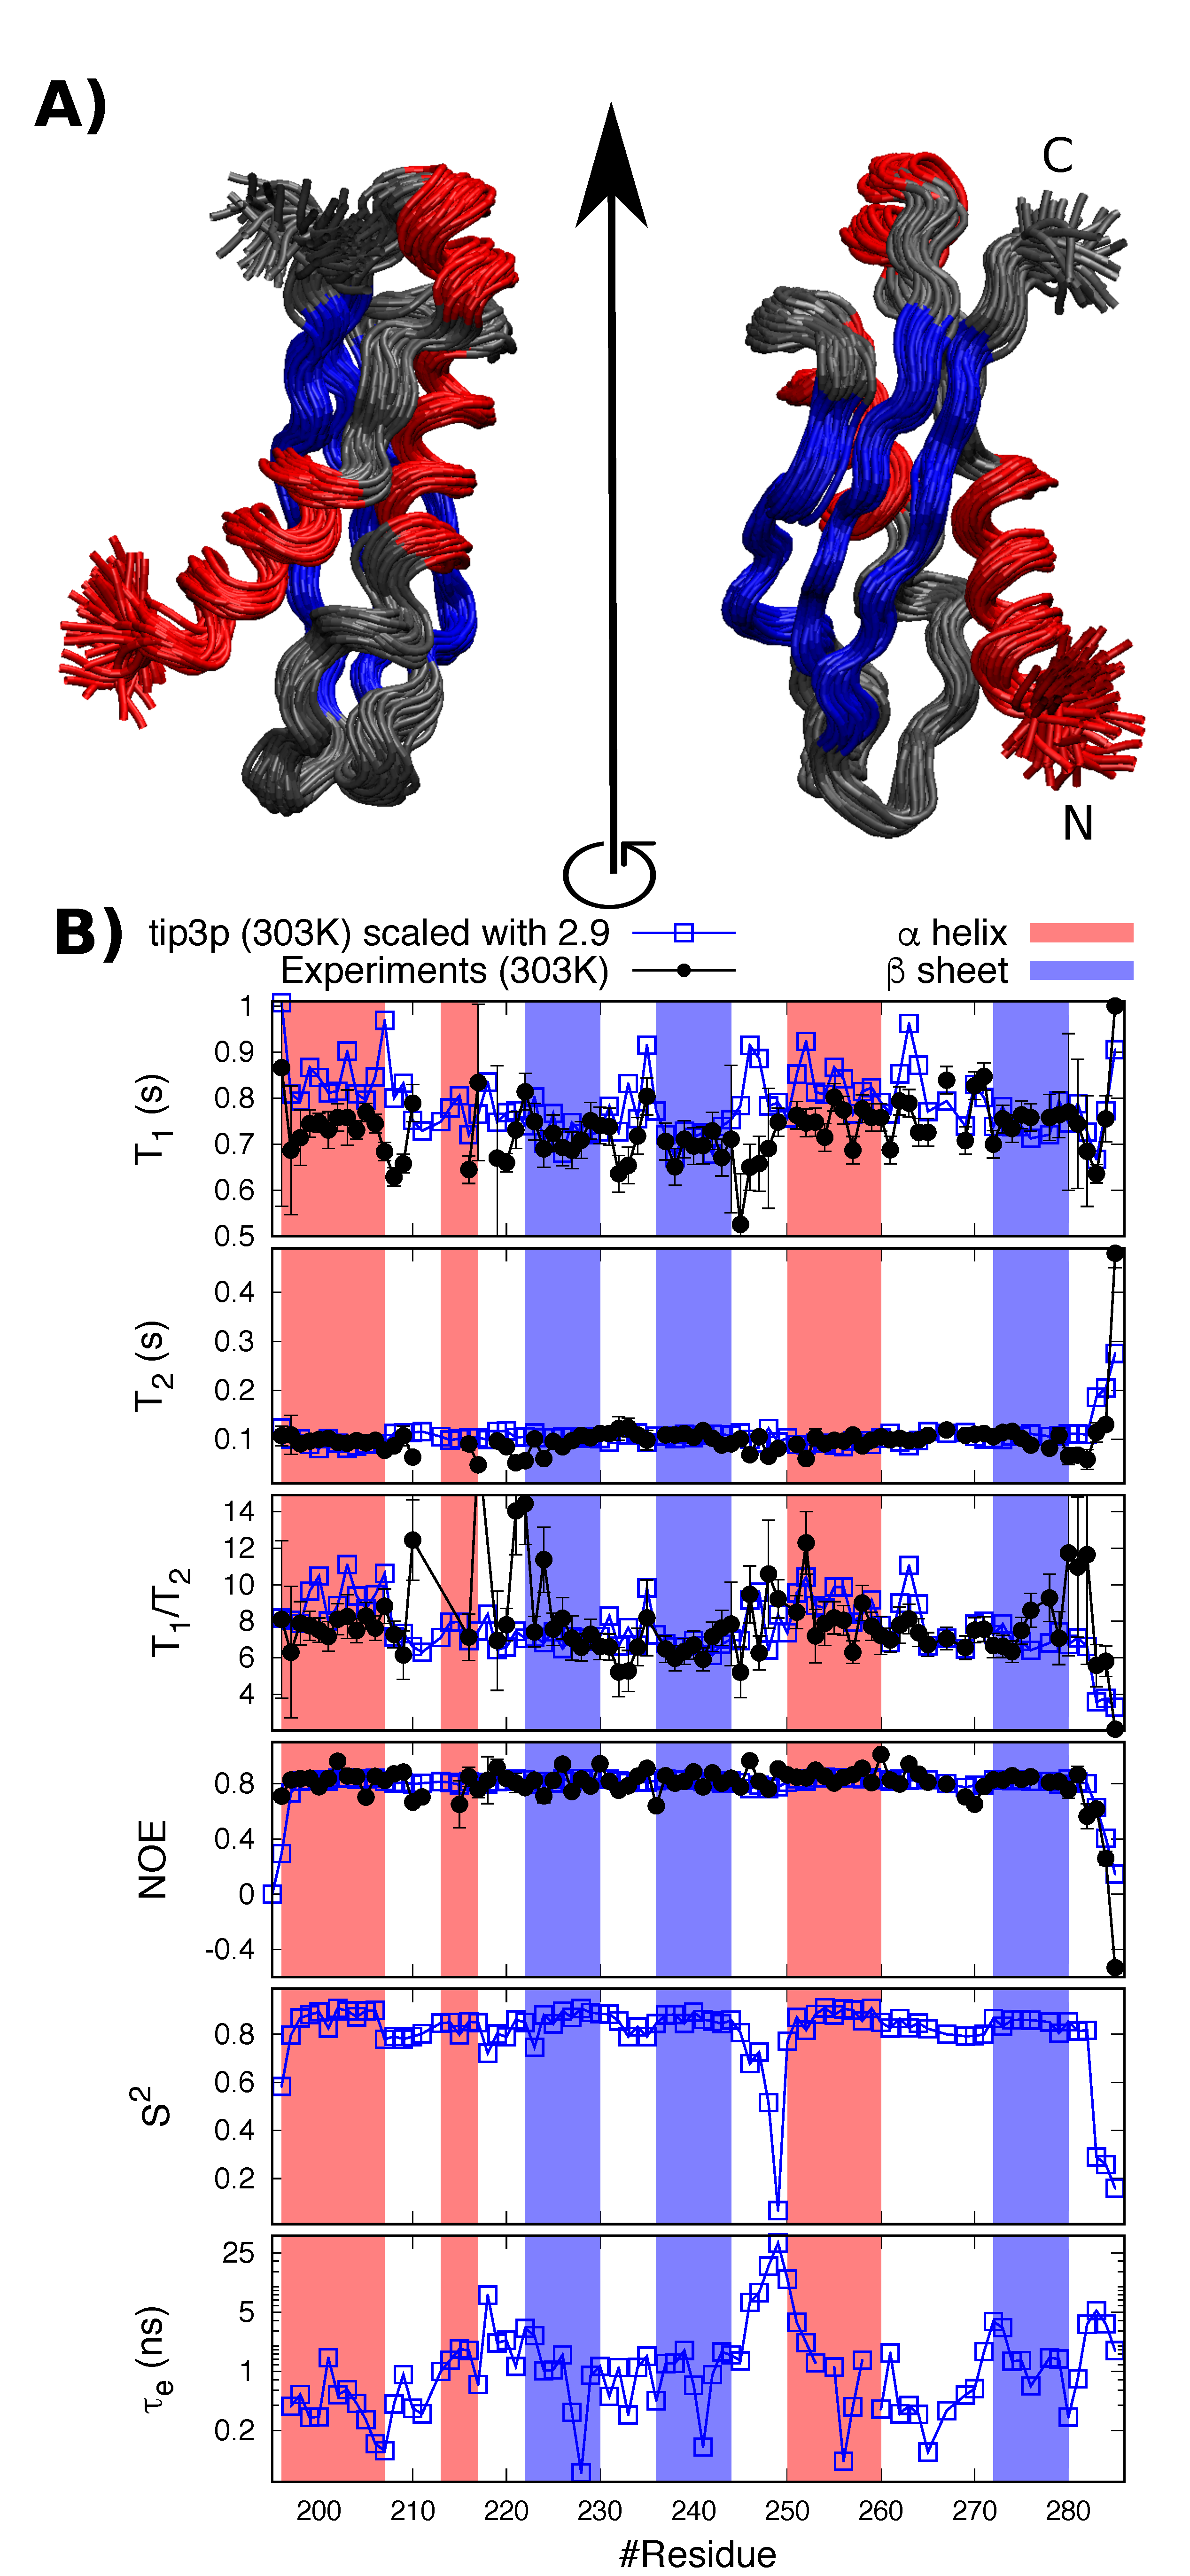
\includegraphics[width=8.5cm]{../Figs/RELdataHpTonB2.eps}%
  \caption{A) Structures of {\it Hp}TonB from the MD simulations with tip3p at 303~K
    (100 structures taken from 400ns long trajectory). Secondary structures
    are colour-labelled with Visual Molecular dynamics \cite{frishman95,humphrey96};
    $\alpha$-helices are red and $\beta$-sheets are blue.
    B) Spin relaxation times from experiments (circles) and tip3p
    simulations (squares) with rotational diffusion coefficients divided by a
    constant factor of 2.9 at 303~K. Order parameters and effective internal correlation
    times calculated from simulations
    \label{HpTonBrelaxationDATAscaled}}%
\end{figure}

Comparison of spin relaxation times between experiments and simulations
with different water models and temperatures
for {\it Pa}TonB construct is shown in Fig. \ref{PsTonBrelaxationDATA}.
Simulations with both tip4p and
OPC4 water models systemically underestimate $T_1$ values
and $T_1/T_2$ ratio when compared with experiments. The discrepancy is,
however, less severe than for {\it Hp}TonB simulated with tip3p in Fig.~\ref{HpTonBrelaxationDATA}. 
Spin relaxation times calculated
%from the new correlation function in Eq. \ref{newCORRF}
after scaling the diffusion coefficients with a constant factor of 1.2
are shown in Fig.~\ref{PsTonBrelaxationDATAscaled} for {\it Pa}TonB simulation with tip4p at 298K.
The results are in good agreement with experiments, suggesting that
the the scaling of overall diffusion constants with a constant factor 
removes the discprepancy with experimental spin relaxation data
also for this system.
Notably, the effect of temperature difference of 12 degrees
on spin relaxation times is significanlty smaller than the difference
between simulations and experiments or the effect of the diffusion constant scaling.
\begin{figure}[!h]
  \includegraphics[width=8.5cm]{../Figs/PsTonBrelaxationDATA.eps}%
  \caption{Spin relaxation times for {\it Pa}TonB from experiments (circles) \cite{??}
    and simulations (squares) with different water models. 
    \label{PsTonBrelaxationDATA}}%
\end{figure}
\begin{figure}[!h]
  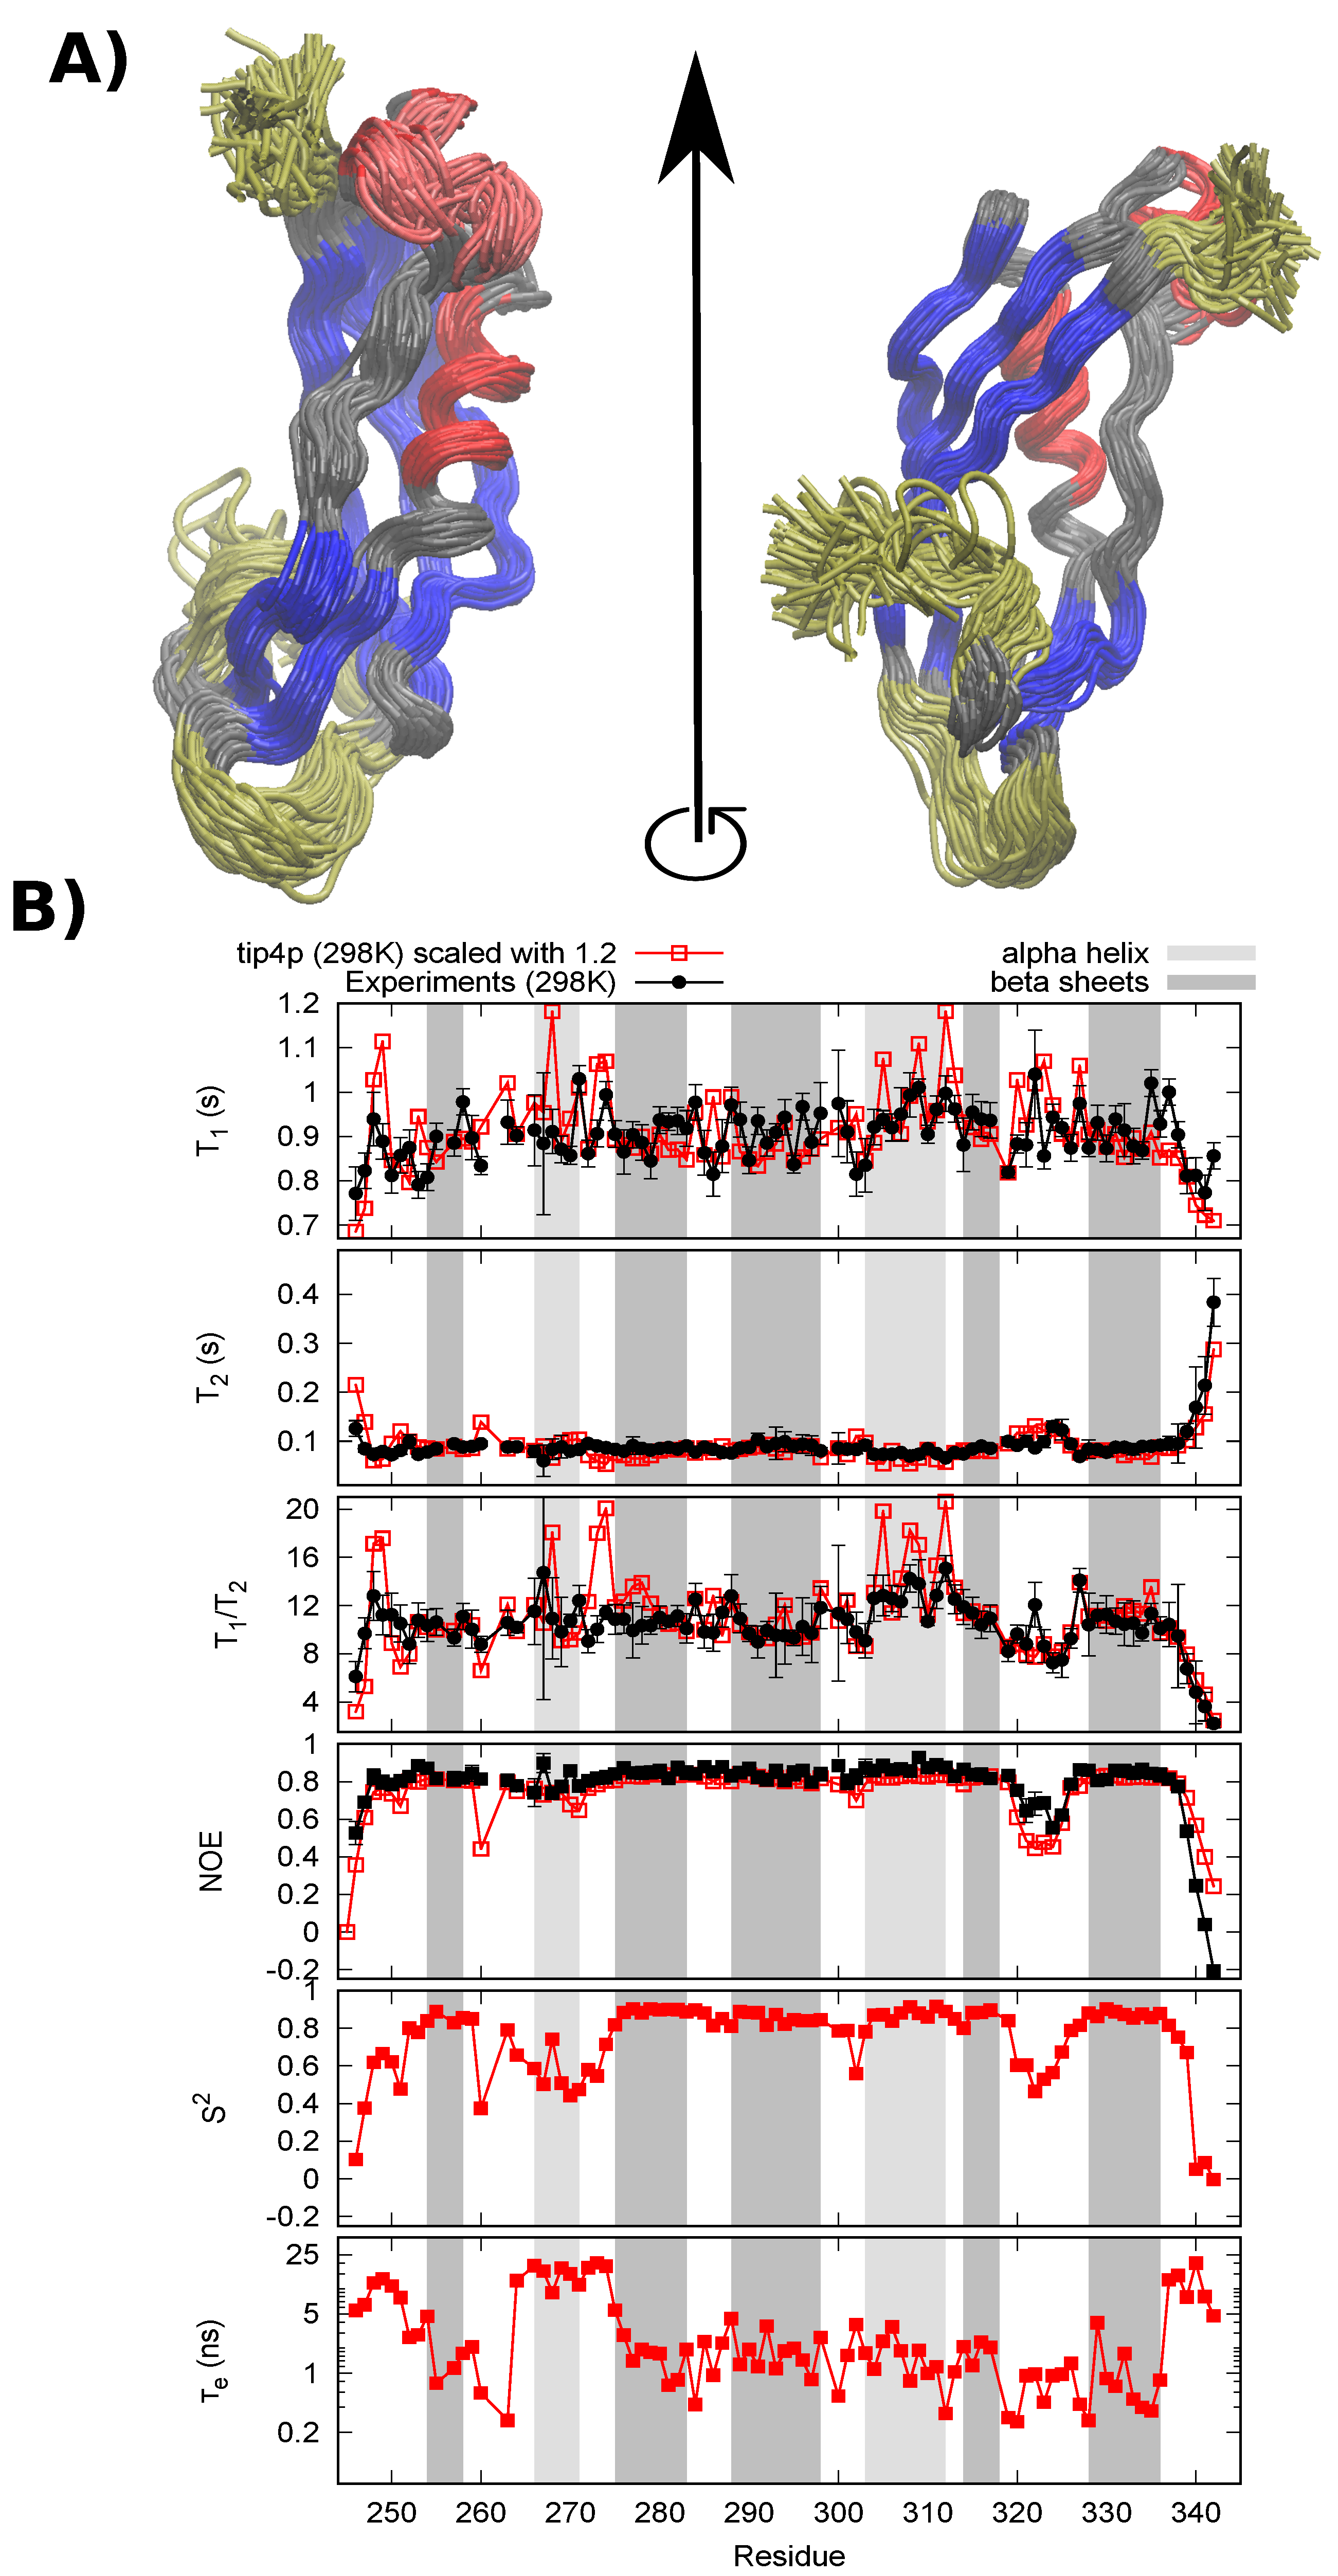
\includegraphics[width=8.0cm]{../Figs/RELdataPsTonB2.eps}%
  \caption{A) Structures sampled by {\it Pa}TonB from MD simulations with tip4p at 298~K
    (100 structures from 400ns long trajectory). Secondary structures
    are colour labelled with Visual Molecular dynamics \cite{frishman95,humphrey96};
    $\alpha$-helixes are red and $\beta$-sheets are blue.
    Residues 246-251, 320-326 and 338-342 with increased internal dynamics are yellow and
    $\alpha$-helix fluctuations between two orientations (residues 266-270) is pink in the left column.
    B) Spin relaxation times from experiments (circles) and tip4p
    simulations (squares) with rotational diffusion coefficients divided by a
    constant factor of 1.2 at 298~K. Order parameters and effective internal correlation
    times calculated from simulations. \label{PsTonBrelaxationDATAscaled}}%
\end{figure}

Simulation data with the scaled diffusion coefficients 
lead to a good agreement with spin relaxation experiments as seen
in Figs.~\ref{HpTonBrelaxationDATAscaled} and~\ref{PsTonBrelaxationDATAscaled}.
This suggests that the scaled diffusion constant values can be used to interpret
the anisotropic diffusion observed in NMR experiments.
The rotational diffusion coefficients giving the best agreement with experimental 
data are collected in Table \ref{ROTdiffCOEFFSscaled}.
%The scaled diffusion coefficients
%from tip3p simulations were chosen for {\it Hp}TonB-92, because they give
%slightly better overall agreement with experiments than simulations with
%tip4p water model.
In contrast to the diffusion constants in Table~\ref{ROTdiffCOEFFS},
these results are in line with previously reported values for more isotropic
proteins~\cite{krishnan98}.
\begin{table}[!h]
  \centering
  \caption{Rotational diffusion coefficients giving the best agreement with experimental spin relaxation data.
    For {\it Hp}TonB construct the values calculated from simulation with tip3p were scaled with 2.9
    (spin relaxation data in Fig.~\ref{HpTonBrelaxationDATAscaled}) and  for {\it Pa}TonB
    the values from tip4p simulation at 298K were scaled by 1.2 (spin relaxation data in
    Fig.~\ref{PsTonBrelaxationDATAscaled}). 
  }\label{ROTdiffCOEFFSscaled}
  \begin{tabular}{c c c c c}
    &    &  {\it Hp}TonB  &  & {\it Pa}TonB \\
    \hline
    $D_{xx}$        &    &   2.15 $\pm$ 0.01  & & 1.51  $\pm$ 0.01\\
    $D_{yy}$        &    &  2.43  $\pm$ 0.01  & & 1.72  $\pm$ 0.03\\
    $D_{zz}$        &    &  4.10   $\pm$ 0.01 & & 3.79  $\pm$ 0.03\\
    $D_{av}$        &    &   2.90  $\pm$ 0.03  & & 2.3  $\pm$ 0.02\\
    $\tau_{c}$(ns)\footnote{$(6D_{av})^{-1}$}  &    &  5.7   $\pm$ 0.1  & & 7.2 $\pm$ 0.1 \\
    $\tau_{c}'$(ns)\footnote{Average over rigid residues given by Eq. \ref{ratioEQ}}  &    &  5.7   $\pm$ 0.1  & & 7.2 $\pm$ 0.1 \\
    %\hline
\end{tabular}
\end{table} 


%\begin{table}[htb]
%\centering
%\caption{Rotational diffusion coefficients (rad$^2\cdot 10^7$/s) calculated from {\it Hp}TonB-92 simulations}\label{ROTdiffCOEFFShp}
%\begin{tabular}{c c c c c c c }
%            &  &  TIP3P  & &   TIP4P   &  &   OPC \\
%  \hline
%  D$_{xx}$   & &   0.083   & &   0.038   &  &   0.030 \\
%  D$_{yy}$   & &  0.077   &    &   0.033   &  &   0.027 \\
%  D$_{zz}$   & &  0.16    &    &   0.059   &  &    0.058 \\
%  2D$_{zz}$/(D$_{xx}$+D$_{yy}$) &  &   1.99    &  & 1.7    &	&  2.03 \\
%  D$_{av}$  &    &   0.11    &    &   0.043   &  &   0.038 \\
%  tau1     &  &  1.76	 &       &   4.13    &   &   4.87 \\
%  tau2     &  &  1.82	 &       &   4.40    &   &   5.14 \\
%  tau3     &  &  1.26	&        &   3.25    &   &   3.47 \\
%  tau4     &  &  1.05	 &       &    2.75   &   &  2.94 \\
%  tau5     &  &  3.05	 &       &    6.48   &   &   8.43 \\
  
  %\hline
%\end{tabular}
%\end{table} 

%Results with rotational diffusion coefficient corrected with constant factor
%are shown in Fig. \ref{relaxationDATAplotSCALED}. 
%\begin{figure}[!h]
%  \includegraphics[width=13cm]{/Users/osollila/Dropbox/TonB/Figs/relaxationDATAplotSCALED.eps}%
%  \includegraphics[width=13cm]{/home/samuli/Dropbox/TonB/Figs/relaxationDATAplotSCALED.eps}%
%  \caption{Relaxation parameters for HpTonB short construct from
%    experiments and simulations with Amber-ildn and different water models.
%    The rotational diffusion coefficients are divided by 3.0 for tip3p simulation
%    and by 1.3 for tip4p simulation.
%    Experiments are done in 303K and simulations in 310K, simulations in 303K are running.
%    \label{relaxationDATAplotSCALED}}%
%\end{figure}

%\begin{figure}[!h]
%  \includegraphics[width=13cm]{/Users/osollila/Dropbox/TonB/Figs/relaxationDATAplotLONGERconstructSCALED.eps}%
%  \includegraphics[width=13cm]{/home/samuli/Dropbox/TonB/Figs/relaxationDATAplotLONGERconstructSCALED.eps}%
%  \caption{PRELIMINARY RESULTS for relaxation parameters for HpTonB longer construct (107) from
%    experiments and simulations with Amber-ildn and tip4p water models.
%    The rotational diffusion coefficients are divided by 1.3.
%    Experiments and simulations are done in 303K.
%    \label{relaxationDATAplotSCALEDlongerCONSTRUCT}}%
%\end{figure}


%\begin{table}[htb]
%\centering
%\caption{Rotational diffusion coefficients scaled with constant factor which
%  gives a good agreement for spin relaxation data,  3.0 for tip3p simulation
%    and by 1.3 for tip4p simulation.
%  OPC RESULTS TO BE CHECKED.
%}\label{ROTdiffCOEFFS}
%\begin{tabular}{c c c c c c c }
%  rad$^2$/ns   &    &  TIP3P  &   &   TIP4P \\%  &  &   OPC \\
%  \hline
%  D$_{xx}$    &   &   0.028   &   &   0.029 \\%  &  &   0.030 \\
%  D$_{yy}$   &    &  0.026   &    &   0.025 \\%  &  &   0.027 \\
%  D$_{zz}$   &    &  0.053    &    &   0.045 \\%   &  &    0.058 \\
%  2D$_{zz}$/(D$_{xx}$+D$_{yy}$) &  &   1.99    &  & 1.7 \\%   &	&  2.03 \\
%  D$_{av}$  &    &   0.034    &    &   0.033 \\%  &  &   0.038 \\
  %\hline
%\end{tabular}
%\end{table} 



\subsection{Interpretation of protein internal relaxation from MD simulations}
Good agreement of spin relaxation times between simulations
with scaled overall rotational diffusion constants and
experiments in Figs. \ref{HpTonBrelaxationDATAscaled} and \ref{PsTonBrelaxationDATAscaled}
suggest that the simulations can be used to interpret the internal
dynamics of proteins observed in the experiments.

Only small variations between different residues are observed
for spin relaxation times of {\it Hp}TonB construct in Fig. \ref{HpTonBrelaxationDATA}.
This indicates a rather rigid protein structure, which is also seen in
MD simulation snapshots overlayed in Fig. \ref{HpTonBrelaxationDATA} A).
Only few residues in the terminal ends show slightly
enhanced conformational fluctuations in MD simulations and in
spin relaxation data. Deviations from average spin relaxation times
are also observed in experiements close to residues 210-222, where also 
difficulties in peak assignment were observed \cite{ciragan16}.
Simulations of {\it Hp}TonB construct do not explain this,
however, similar region in {\it Pa}TonB simulation shows 
fluctuations between two orientations of $\alpha$-helix (see discussion below).
Residues 245-250 in {\it Hp}TonB give exceptionally low order parameters
and long effective correlation times in simulations and small $T_1$ times
in experiments. The interpretation of this is, however, not straightforward,
because low $T_1$ values in this region are not reproduced by MD simulations.
%More detailed discussion together with
%longer {\it Hp}TonB construct is presented elsewhere \cite{??}.

More variety in internal dynamics between residues is observed for {\it Pa}TonB
protein
%in Fig. \ref{PsTonBrelaxationDATAscaled}.
and segments with enhanced conformational fluctuations are labelled with yellow colour
in Fig. \ref{PsTonBrelaxationDATAscaled}.
Larger number of sampled conformations in both terminal ends
%show significantly enhanced conformational fluctuations
%in MD simulations and in spin relaxation experiments. The terminal ends
are characterized by low order parameters and long effective internal correlation times
observed in simulations. 
Enhanced conformational fluctuations is also observed for residues between 320-326,
which is a loop between two $\beta$-sheets.
MD simulations predict low order parameters and long internal effective correlation
times also for residues between 260-274. These can be explained by  
two different orientations sampled by the $\alpha$-helix in this region
(colour labelled with pink in Fig.~\ref{PsTonBrelaxationDATAscaled} A).
The orientational fluctuations of the similar short helix could also explain 
lower spectral resolution and deviations in spin relaxation times
observed for residues close to residue 210-222 in {\it Hp}TonB~\cite{ciragan16}.

MD simulations can be used to suggest how rotational dynamics of N-H bonds
builds up from different components. Here we fit a sum of 471 different
timescales to the correlation functions according to Eq.~\ref{gprime_fit}.
Most prefactor values are zero in all correlation functions in this work,
thus the remaining timescales with non-zero prefactors are considered as different
components of the total relaxation process.
The prefactors are shown in Fig. \ref{coeffsPLOT} for the same residues
of {\it Pa}TonB, which were used to exemplify correlation functions in Fig. \ref{exampleCORRF}.
As expected for residue 322 in rigid $\beta$-sheet with large order parameter value,
the rotational relaxation is dominated by timescales of $\sim$5.5~ns and $\sim$8~ns,
matching with protein overall
rotation. Also the dynamics of the selected residue 322 in flexible loop is
dominated by timescales around $\sim$8~ns corresponding protein overall rotation,
however, fast motions from internal dynamics are more significant than for the
rigid $\beta$-sheet residue. This is in agreement with lower order parameter value
in the flexible loop residues. On the other hand, the rotational dynamics of
the selected residue 341 in the flexible N-terminus is dominated by timescales
below 3~ns, most likely related to the internal protein dynamics.
The contribution from timescales close to $\sim$13~ns probably
arises from slow conformational fluctuations of N-terminus, rather than overall
rotational dynamics. This supports the conclusion that fluctuations of large amount of
conformations leads to small order parameters and large effective correlation times
observed in Fig. \ref{PsTonBrelaxationDATA}.
While fractionalization of rotational dynamics to different components
gives intuitively understandable results, it should be kept in mind that
it is based on fitting of multiexponential sum to the simulation data and the solution
of such fit is not unique.
\begin{figure}[!h]
  \includegraphics[width=8.5cm]{../Figs/coeffsPLOT.eps}%
  \caption{Prefactors $\alpha_i$ corresponding different timescales $\tau_i$
    resulting from a fit of Eq.\ref{gprime_fit} to correlation functions from
    MD simulation of {\it Pa}TonB at 298K. The used correlation functions give
    a good agreement with experimental spin relaxation times as shown in
    Fig.~\ref{PsTonBrelaxationDATAscaled}.  \label{coeffsPLOT}}%
\end{figure}



\section{Discussion and conclusions}
Experimental spin relaxation data for protein backbone N-H bonds
was successfully reproduced by using classical molecular dynamics
simulations for two different proteins with anisotropic molecular
shape. Thus, the simulation trajectories give an atomic resolution
interpretation for the protein dynamics measured with NMR experiments.
Interpretation of overall and internal dynamics was demonstrated for
two relatively rigid proteins. The proposed approach is expected
to be especially useful in the interpretation of spin relaxation data
of proteins containinig some interesting flexible domains and having
an anisotropic shape. Interpretation of relaxation data measured from
such proteins has been very challenging with the previously available
methods~\cite{barbato92}.


Direct analysis of classical molecular dynamics trajectories did not, however,
reproduce the experimental data. Comparison of calculated diffusion constants
%, calculated from the slope of mean square angle deviations of inertia axes (Eq. \ref{DIFFdef}),
and spin relaxation times with experimental data suggested that
the overall brownian tumbling of protein is too rapid in simulations,
in agreement with previous studys suggesting that the discrepance arises
from the inaccuracies in water models~\cite{wong08}.
Scaling down the diffusion coefficients in simulation data
with the same factor in all directions 
led to good agreement with experiments and allowed the interpretation.
The overall rotation of proteins was found to be brownian having
only a small subdiffusive behaviour with short timescales
below~$\sim$0.12 ns. This can be constrasted with crowded environments,
where anomalous diffusion is expected to be more significant \cite{hofling13}.
%which were found to be essentially linear for all inertia axes.
%The results indicate that monomeric proteins in dilute solution
%experience rotational brownian tumbling 

Similarity between correlation functions from the original MD trajectory and
the new correlation functions from Eq.~\ref{newCORRF} 
%General form of rotational correlation function for anisotropic rigid body
%(Eq.~\ref{CORRFanisot}) with timescales from rotational diffusion constants
%was successfully fit to the overall rotational correlation functions from
%MD simulations for all individual N-H bonds.
%Furthermore, the new correlation
%functions calculated from Eq.~\ref{newCORRF} were in good agreement with
%the total correlation functions calculated from original trajectories.
suggest that the usage of intertia axes
%can be used to describe
%the overall rotational diffusion as a good approximation
and the separation of internal and overall rotational motions
(Eq.~\ref{CORRFsep}) are good approximations for the investigated
proteins. However, rather rigid proteins are studied in this
work and in previous publications with similar conclusions~\cite{wong08,allner15}.
These assumptions become less rigorous for proteins with larger
fractions of intrinsically disoredered segments. In such cases the option
might be to use isotropic reorientational eigenmode dynamics (iRED)~\cite{prompers02}
or quaternions~\cite{anderson12}. However, the correction of the overall
rotational diffusion artefact due to the inaccurate water model would be complicated
for intrinsically ordered molecules in all the discussed approaches.
Thus, a water model giving correct
overall rotational diffusion rates for biomolecules is probably necessary
to compare simulations of intrinsically disordered molecules
to experimental spin relaxation data.

%Usage of the new correlation functions from Eq.~\ref{newCORRF} in
%spin relaxation time calculations reduces the statistical fluctuations
%with long lag times in correlation function calculation,
%which allows the higher accuracy with less simulation data.
%The essential reason is that the rotational diffusion constants
%can be determined by fitting a single parameter (linear slope) which is
%more robust than a direct fit of multiexponential correlation function
%to MD simulation result. After determining
%the diffusion constants and using Eq.~\ref{newCORRF},
%the contribution from overall rotation do not have statistical
%fluctuations in correlation functions used in spin relaxation time calculations.

Overall rotational diffusion coefficients were overestimated by a factor of $\sim$3 in
{\it Hp}TonB simulations with tip3p water model, in agreement with previous
studies \cite{prompers02,wong08,anderson12}. Simulations with tip4p and opc4
water models gave spin relaxation times in reasonable agreement with experiments
with scaling factors of $\sim$1-1.2, which is significantly less than for tip3p.
It should be noted, however, that the correct scaling factor for tip4p seems to slightly
different for {\it Hp}TonB and {\it Pa}TonB suggesting that the correction
is not fully determined by bulk water properties. Thus, the role of hydration layer
and water-protein interactions in rotational dynamics is also expected to
be significant.



%The realistic overall rotational dynamics was determined by
%scaling the diffusion coefficients to all directions post-simulationally by the
%same constant factors such that the calculated $T_1/T_2$ was in optimal
%agreement with experiments.



%or correcting overall rotation by using quaternions \cite{anderson12} or
%fitting timescales to satisfy experiments \cite{prompers02} or
%These approaches are not, however, useful for anitropic proteins and order
%parameter comparison is not direct comparison between simulations and experiments in
%the case of freely rotating molecules. 

%, which resulted scaling factor of 1.2 for
%PsTonB simulation with tip4p and factor 2.9 for HpTonB with tip3p.
%The overstimated overall diffusion
%coefficient can be corrected post-simulationally to compare internal dynamics
%and order with experiments. 
%As already observed previously
%In addition, diffusion constants can be scaled with a constant
%factor before calculating the new correlation functions to compensate
%the overestimated rotational diffusion due to inaccuracies in some
%water models.

%A good agreement between spin relaxation times from experiments and simulations is
%found after overall rotational diffusion constants are scaled with a constant
%factor. This allows the interpretation of internal protein dynamics
%from spin relaxation times by using MD simulations even with tip3p water model.
%Here we use the approach to indentify dynamical regions in two proteins,
%{\it Hp}TonB-92 and {\it Pa}TonB with relatively rigid structures. However, the
%approach could be useful for intepretation of spin relaxation data from
%proteins with more regions containing complicated local dynamics, like
%Calmodulin~\cite{barbato92}.


% If you have acknowledgments, this puts in the proper section head.
\begin{acknowledgments}
% Put your acknowledgments here.
  %OHSO acknowledges Aalto science IT project and
  We acknowledge CSC-IT center for science for computational resources %, and Emil Aaltonen foundation for funding.
\end{acknowledgments}

% Create the reference section using BibTe
\bibliography{refs.bib}

%\newpage
%\appendix
\begin{center}
{\bf SUPPLEMENTARY INFORMATION}
\end{center}
\begin{figure*}[!h]
  \includegraphics[width=16.5cm]{../Figs/RMASDplotPsTonBtip4pT310K.eps}%
  \caption{The intertia tensor angles as a function of time and mean square angular
    deviations for {\it Pa}TonB simulation with tip4p water model at 310K.
    \label{RMASDplotLOG310}}%
\end{figure*}
\begin{figure*}[!h]
  \includegraphics[width=16.5cm]{../Figs/RMASDplotPsTonBtip4pT298K.eps}%                                                                                                    
  \caption{The intertia tensor angles as a function of time and mean square angular
    deviations for {\it Pa}TonB simulation with tip4p water model at 298K.
    \label{RMASDplotLOG298}}%                                                                                                                                                  
\end{figure*}


%\todolist
\end{document}
%
% ****** End of file aiptemplate.tex ******
